\section{Grid Study}
Solver Parameters:
\begin{description}[noitemsep]
    \item[Timestepping Scheme:] Euler Explicit
    \item[CFL:] 0.4
    \item[Spatial Scheme:] Scalar Dissipation ($\epsilon = 0.3$)
    \item[\pexit:] $0.72 p_t$
\end{description}

Results are shown in~\Cref{fig:q3}. It can be seen that shock, which is barely
noticeable for number of grid points ($N$) equal to 25, gradually gets sharper as $N$
increases. However, the location of the shock does not really change for $N \ge 50$.
The lack in shock sharpness is due to dissipation errors, which decreases with
reductions in $\Delta x$ -- or increases in $N$, and thus refining the grid
leads to smaller dissipative errors.

Refining the grid increases the number of iterations required to converge. This is
expected for two reasons:
\begin{enumerate}
    \item The timestep $\Delta t$ is proportional to $\Delta x$. Thus, reducing
        $\Delta x$ also requires reducing $\Delta t$ in order to have a stable
        convergence and accurate solution.
    \item Increasing the number of grid points increases the time taken for information
        to travel from one end of the grid to the other. This is amplified by the fact
        that both the inlet and outlet are subsonic and change at every time step.
\end{enumerate}

Total pressure loss is tabulated in~\Cref{tab:q3}. The total pressure loss increases
as the grid is refined. This makes sense from a physical standpoint,
since the shock occurs further, and thus at higher Mach number, as $N$ increases;
shocks at higher Mach numbers are stronger.
\begin{table}[H]
    \centering
    \caption{Total pressure loss for various grid sizes}\label{tab:q3}
    \input{table_q3_ploss}
\end{table}
It can be said
that the shock is in fact a normal shock by comparing the
total pressure loss, which is due to the shock, with the normal shock tables from Fluids 2.
The Mach number at which the shock occurs for the finest grid is around 1.34; according
to the tables this should lead to a total pressure ratio of 0.9718.

Finally, let's look at how the minimum $\epsilon$ required to converge is affected by $N$.
These results are tabulated in~\Cref{tab:q3_eps}. It can be seen that a higher $\epsilon$ is
required as $N$ increases. Recall that decreasing $N$ decreases dissipation errors due to the
spatial discretization and, from Question 2, that a certain amount of dissipation is required
for the solve to converge. Then, decreasing $N$ requires increasing artificial
dissipation through $\epsilon$ to compensate for the decrease in numerical dissipation
error.

\begin{table}[H]
    \centering
    \caption{Minimum allowable $\epsilon$ as a function of $N$.}\label{tab:q3_eps}
    \input{table_q3_eps}
\end{table}
\begin{figure}
    \centering
    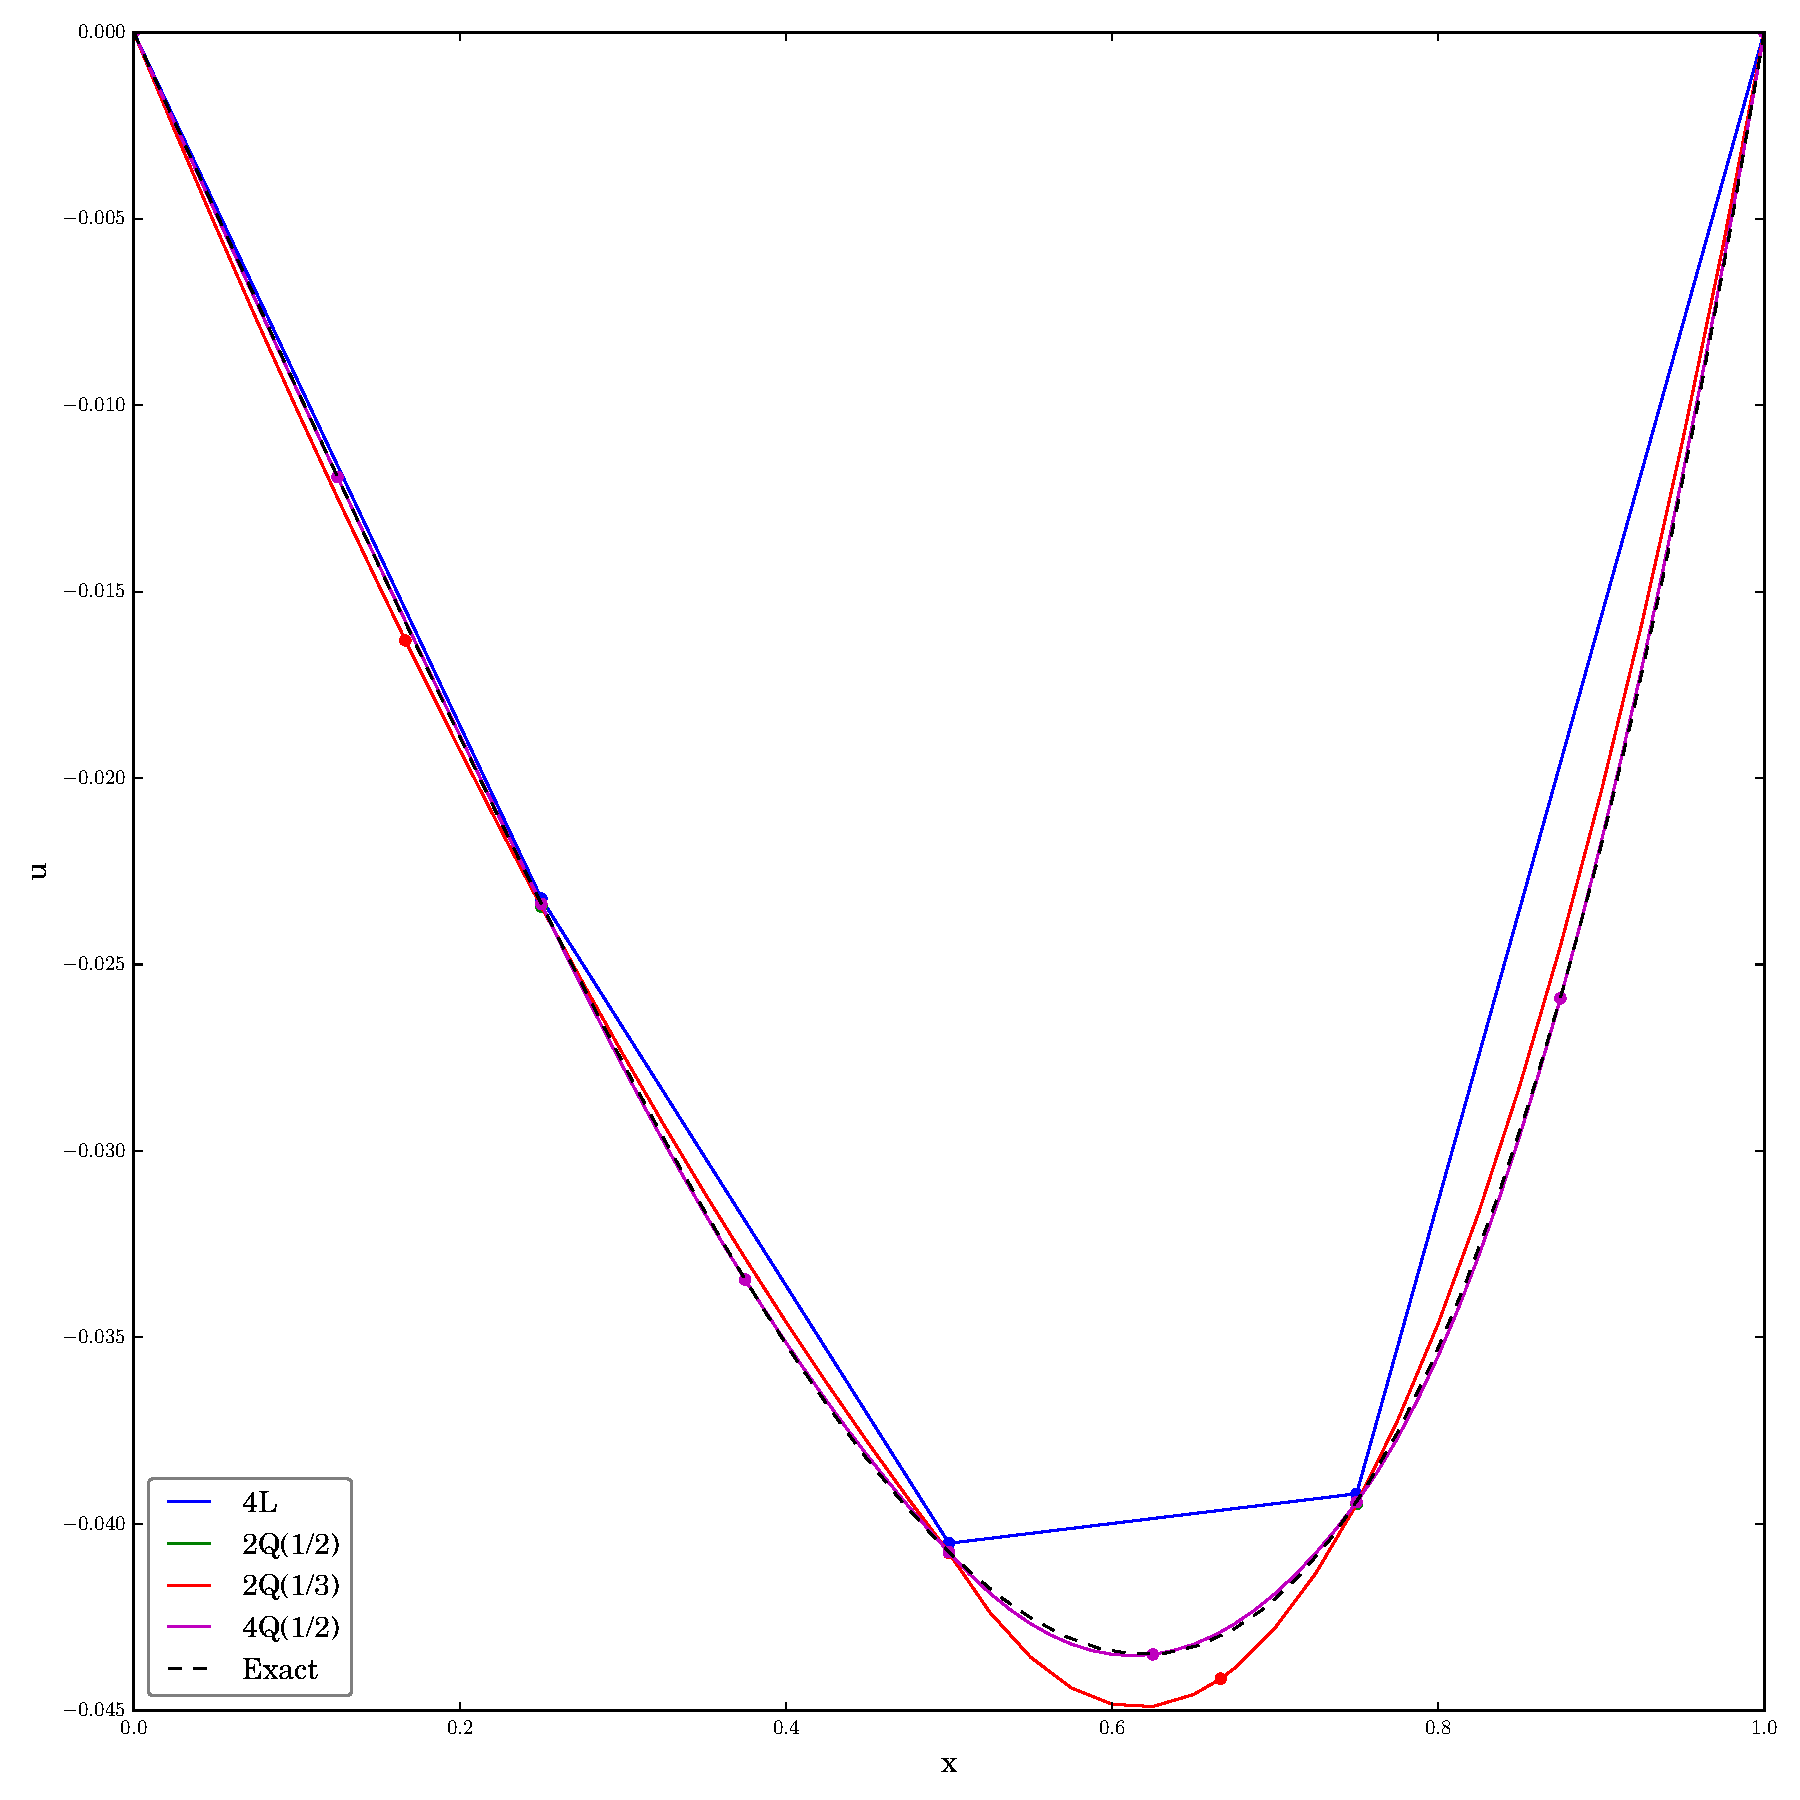
\includegraphics[width=0.9\textwidth]{./figs/q3}
    \caption{Results at $\pexit = 0.72p_t$ for various grid sizes $N$.}\label{fig:q3}
\end{figure}


